\documentclass{article}
\usepackage[a4paper, margin=1.5in]{geometry}
\usepackage[utf8]{inputenc}
\usepackage[T1]{fontenc}
\usepackage{hyperref}
\usepackage{palatino}
\usepackage{listings}
\usepackage{graphicx}
\usepackage{booktabs}

\lstset{language=ML}
\lstset{basicstyle=\footnotesize\ttfamily,breaklines=true}

\title{Extending MLKit with vector instructions}
\author{Christian Kjær Larsen}


\begin{document}

\maketitle

\tableofcontents

\section{Introduction}

In this section we will briefly describe the project, its purpose and the structure of this report.

\subsection{Project statement}

The goal of this project is to add packed vector support to the MLKit\cite{mlkit} Standard ML compiler using the AVX2 vector instructions present in modern Intel processors. The motivation is to be able to use this support to optimize programs written in Standard ML to exploit data parallism.

\subsection{Roadmap}

\begin{enumerate}
    \item We start by investingating other approaches to SIMD programming in higher level languages. This is in order to settle on a
        good abstraction that is fairly easy to program with.
    \item
        We then continue by designing a programming abstraction to be able to optimize a program in a generic way that is not tied to a particular instruction set or vector extensions.
        We also write some simple example programs that will work as motivating examples and show that the abstraction is actually useful.
    \item
        Finally we implement compiler support for Intel AVX in the MLKit Standard ML compiler by providing a set of intrinsics that compile to efficient code that use native vector instructions.
\end{enumerate}

\section{Background}

\subsection{Vector instructions in modern CPUs}

Single instruction stream, but it works on multiple independent pieces of data.

Fewer data dependencies and fewer instructions to be decoded.

MMX, SSE and AVX in Intel processors.

Neon on ARM processors.

\subsection{Programming model and higher level languages}

\subsubsection{Intrinsics}

The primary way that people program with vector instructions is by using intrinsics.

Intrinsic functions for C/C++ guaranteeing what code is generated when the functions are called.

\subsubsection{Rust}

Standard interface to generic functions that are lowered directly to LLVM and compiled for specific architectures there.
\url{https://github.com/rust-lang/stdsimd}

Supposed to be portable, so you can write a function that works for vectors of, say, 4 64-bit floats, and then it would be lowered to the LLVM type \verb!<4 x double>!. The problem of choosing good instruction for certain operations are then delegated to the LLVM backend.

\subsubsection{.NET and Java}

\url{https://docs.microsoft.com/en-us/dotnet/api/system.numerics.vector?view=net-5.0}


\subsubsection{Challenges}

One major challenge is not to tie the implementations to tightly to the specific instruction set. It should be fairly easy to change a program from say AVX2 to Neon. This then gives the problem of instruction selection. Do you expose direct versions of the AVX2 instructions, and then make other instruction sets emulate those, or do you try to find a common ground, that makes useful operations with good performance available on all CPUs.

Take for instance a horizontal add,
\[
    \mathtt{hadd}\ [a_1, \ldots, a_4] = a_1 + \cdots + a_4
\]
for reducing a 4 element vector. The AVX2 instruction set has no direct support, and the most efficient implementation might depend on vector sizes and element types. The proposed RISC-V vector extensions directly expose a \texttt{vfredsum.vs} that directly reduces a vector.

Since we in this project only focus on MLKits 64 bit intel backend, we restrict ourselves to vectors of reals (64 bit floats) of 4 elements. This is supported by AVX2 which is widely supported now. We will of course keep in mind to design our library such that it is not too tied to AVX2.

\section{Design of a vector signature}

In this section we will briefly describe a vector signature that can be used for SIMD programming in SML. We will also show how to write simple programs that use it.

\subsection{Generic interface}

We have created a \verb!REAL4! signature that will operate on a packed vector of 4 \verb!real!s. An overview can be seen on listing~\ref{lst:real4}.

\begin{lstlisting}[frame=single, caption=\texttt{REAL4} vector signature, label={lst:real4}]
signature REAL4 = sig

  type element = real
  type interface = real * real * real * real

  type simd
  type mask

  val mk : interface -> simd
  val read : simd -> interface

  val broadcast : element -> simd

  (* arithmetic operations (vectors and scalars) *)
  val add : simd * simd -> simd
  val adds : simd * element -> simd
  (* and so on *)

  (* comparisons (vectors and scalars) *)
  val lt : simd * simd -> mask
  val lts : simd * element -> mask
  (* and so on *)

  (* operations on masks *)
  val and_ : mask * mask -> mask
  val or_ : mask * mask -> mask
  val not_ : mask -> mask

  (* reductions *)
  val all : mask -> boolean
  val any : mask -> boolean
  val sum : simd -> element
  val product : simd -> element

  (* conditional operations *)
  val blend : simd * simd * mask -> simd
end
\end{lstlisting}

There are two opaque types. \verb!simd! represents the actual vector and \verb!mask! represents a vector of booleans that can be the result of comparisons. We have chosen to fix the number of elements in the signature, since this makes the signature much easier to use. An alternative would be to make the \verb!mk! and \verb!read! functions work on lists, and then we could reuse the signature to work on multiple vector lengths. This of course makes the interface more fragile.

We include arithmetic operations both in vector-vector and vector-scalar form. The comparisons will return masks where the individual elements correspond to the comparison between individual elements. We also include common boolean operations on masks.

To collapse vectors into elements, we also include some reductions. Sum and product of vectors will collapse an entire vector into the sum or product of its elements. \verb!all! and \verb!any! will return true if all or any of its elements are true. Other reductions could also be added in the future like minimum and maximum.


A signature for packed integers \texttt{INT4} could also be added, and an implementation could also be made using AVX2 instructions, but we have chosen to focus on floating point in this project. It would of course include different operations more specific to integers.

\subsection{Pure SML structure}

It is pretty easy to implement a pure SML structure that we can use to test our hardware accelerated version against. We just use tuples of reals for vectors and tuples of booleans for masks.
\begin{lstlisting}[frame=single, label={lst:tup4}, caption={Implementation of \texttt{REAL4} using tuples}]
structure Tup4 : REAL4 = struct
  type simd = real * real * real * real
  type mask = bool * bool * bool * bool

  fun mk a = a
  fun read a = a

  fun broadcast v = (v, v, v, v)
  fun all (m1, m2, m3, m4) = m1 andalso m2 andalso m3 andalso m4

  (* And so on *)
end
\end{lstlisting}

\subsection{Writing programs}

Writing a simple numeric program is very simple, since the \verb!simd! values are almost interchangable with reals.
\begin{lstlisting}[frame=single, label={lst:numeric}, caption={Numeric program}]
fun foo (x: real, y: real) = x*x + y*y
fun foo_simd (x: simd, y: simd) = add (mul (x, x), mul (y, y))
\end{lstlisting}
We can write programs with conditionals by using the \texttt{blend} operation. It gives us the possibility to select from one of two vectors based on a mask. We can use it to write a vectorized version of a maximum function:
\begin{lstlisting}[frame=single, label={lst:max}, caption={Max function}]
fun max (v1: real, v2: real) = if v1 < v2 then v2 else v1

fun max_simd (v1: simd, v2: simd): simd =
  blend (v1, v2, lt (v1, v2))
\end{lstlisting}
\texttt{blend} will select elements from the first vector when the element in the mask is true, and otherwise take the element from the second vector.

If we want to write a loop that terminates based on some condition about elements of the vector, we can use the boolean reductions to make a predicate about the entire vector.
We can for instance make a tail recursive function that adds 1.0 to each element until all elements are above 9000.
\begin{lstlisting}[frame=single, label={lst:max}, caption={Iteration with guard}]
fun loop (x: simd): simd =
  if all (gts (x, 9000.0))
    then x
    else loop (adds (x, 1.0))
\end{lstlisting}

\subsubsection{Vectorizing mandelbrot}

Using these building blocks, we can try to rewrite a larger program to use the vectorized operations. We will take a look at a simple implementation of a function that calculates whether a complex number belongs to the Mandelbrot set.
\begin{lstlisting}[frame=single, label={lst:scalar_mandel}, caption={Scalar Mandelbrot}]
fun mandelbrot (re: real, im: real): int =
  let
    fun go iter x y =
      if (re*re + im*im <= 4.0 andalso iter < 1000)
      then go (iter + 1) (re*re - im*im + x0) (2.0*re*im + y0)
      else iter
  in
    go 0 0.0 0.0
  end
\end{lstlisting}
A way to approach it is to consider 4 values $(x_1, y), \ldots, (x_4, y)$. The problem is that for 4 pixels it might be the case that some diverge and some converge. We can use masks to essentially block the updates for pixels that have converged already.

\begin{lstlisting}[frame=single, label={lst:vector_mandel}, caption={Vector Mandelbrot}]
functor Mandelbrot(Real4 : REAL4) = struct
open Real4
fun mandelbrot_simd (re: simd, im: real): simd =
  let
    val zero = broadcast 0.0
    fun square x = mul (x, x)
    fun go (iter, iters, re', im') =
      let
        val re2 = square re'
        val im2 = square im'
        val mask = les (add (re2, im2), 4.0)
      in
        if (any mask andalso iter < 1000)
        then
          let 
            val re'' = add (sub (re2, im2), re)
            val im'' = adds (muls (mul (re', im'), 2.0), im)
          in
            go ( iter + 1
               , blend (iters, adds (iters, 1.0), mask)
               , blend (re', re'', mask)
               , blend (im', im'', mask)
               )
          end
      else iters
    end
  in
    go (0, zero, zero, zero)
  end
end
\end{lstlisting}
We start by computing the mask that corresponds to the condition in the original if-statement. If all values are false, we stop iterating, since all values in the vector has either converged or diverged. We then use the \verb!blend! operation to conditionally update only the iteration count and the temporary values for those elements where the if-condition in the original program would have been true.

Rewriting a program like this is a bit mechanical, and could maybe be done automatically for these kinds of functions with some meta-programming.

\section{Implementation in the MLKit}
In this section we will describe the changes made to the MLKit compiler in order to support the vector operations described in the precious section using AVX2 instructions. The internals of the MLKit is not super documented, so there will be a lot of mentions of concepts in the compiler that has no references, and is simply understood by reading through the codebase.

\subsection{Primops}
The way that the programmer will have access to native vector instructions is through the \texttt{prim} feature of MLKit. 

On table~\ref{tbl:primops} an overview of the added user facing primops can be seen.

\begin{table}
\begin{tabular}{ l l l }
    \toprule
    Category & Primop & Type \\
    \midrule
    Artithmetic & \verb!__m256d_plus! & \verb!string * string -> string! \\
                & \verb!__m256d_minus! & \verb!string * string -> string! \\
                & etc. & \\
                \midrule 
    Logic       & \verb!__m256d_and! & \verb!string * string -> string! \\
                & \verb!__m256d_not! & \verb!string -> string! \\
                & etc. & \\
                \midrule 
    Conditional & \verb!__m256d_le! & \verb!string * string -> string! \\
                & \verb!__m256d_blend! & \verb!string * string * string -> string! \\
                & etc. & \\
                \midrule 
    Reductions  & \verb!__m256d_all! & \verb!string -> bool! \\
                & \verb!__m256d_sum! & \verb!string -> real! \\
                & etc. & \\
                \midrule 
    Load and store & \verb!__m256d_broadcast! & \verb!real -> string! \\
                   & \verb!__m256d_true! & \verb!unit -> string! \\
                   & \verb!__blockf64_update_m256d! & \verb!string * int * string -> unit! \\
                   & \verb!__blockf64_sub_m256d! & \verb!string * int -> string! \\
                   & etc. & \\
                   \bottomrule
\end{tabular}
\caption{Overview of added primops}
\label{tbl:primops}
\end{table}

We steal the naming convention from Intel that \texttt{m256d} is a 256 bit vector of double precision floating point numbers. The user facing type of vectors is \verb!string! which is chosen, since in the compiler it is a type that roughly corresponds to an array of bytes. We can hide this type in a structure which implements the \texttt{REAL4} signature by using opaque signature matching, so that the user does not accidentally concatenate it with another string.

Most of these operations correspond directly to the functions in the \texttt{REAL4} signature. Additionally we have added primops for dealing with unboxed arrays of reals. The \verb!__blockf64_update_m256d! primop will update 4 values at the specified index in a block of memory containing unboxed reals. The \verb!__blockf64_sub_m256d! will get the 4-element vector from the specified index.

    
\subsection{Internal representation}

2. add unboxed internal representation and make operations for boxing and unboxing. Change the backend to use vector registers for some operations.

Since Standard ML is polymorphic, there might be polymorphic functions that can receive arguments of any type. This is typically achieved by having a uniform representation of values. Typically a box (pointer to the underlying data). There is a substantial penalty for this, since in order to do operations on the underlying value, there is a level of indirection. For our new vector type we will have to use 16 bytes of memory in addition to the pointer to represent something that typically fits in a register.

Any operation that works on a boxed representation will typically have to unbox the data, do the operation and box the result again. This is very costly on modern hardware.


The MLKit has a boxed floating point representation accessible to the programmer as the \verb!real! type in Standard ML. Internally in the optimizer, unnessecary boxing operations are avoided by using unboxed operations directly on floating point registers thereby avoiding expensive memory operations in basic blocks. Due to the uniform memory represenation, these unboxed floats can not be passed to generic functions and should therefore not be exposed to the programmer.

We will do something similar for our vector representation. A boxed representation will be visible to the programmer, but internally a \verb!F256! type will be used to represent a register containing 4 64-bit floating point numbers.

f256 for the unboxed type.

\subsection{Implementing boxed operations}

Take all the operations in table~\ref{tbl:primops} and make unboxed versions that operate on the internal \verb!f256! and \verb!f64! types and the and insert explicit boxing operations around the result, and unboxing operations around the arguments. Roughly speaking we want the following equivalence
\[
    f_{\mathrm{boxed}} \equiv \mathtt{box}\ (f_{\mathrm{unboxed}} (\mathtt{unbox}\ x))
\]
to hold.

Then we only have to implement support for unboxed operations, and the complexity of dealing with memory allocation, loading and storing vector values to memory will be handled in one location.

For boxing we will make two primops \verb!__f256_box! and \verb!__f256_unbox!.

\paragraph{Unboxing}
The unboxing operation will just load the vector from memory using a \verb!vmovupd! instruction.

\paragraph{Boxing}
The boxing operation is a bit more complicated. We will not generate code for the boxing operation. What we will do instead is to rewrite the boxing operation to the following code in the last step of the optimizer:
\begin{lstlisting}
let
  val box = alloc_vector ()
  val ()  = store_vector (value, box)
in box
\end{lstlisting}
Where the two \verb!alloc_vector! and \verb!store_vector! will be distinct primops. \verb!alloc_vector! will use the \verb!SCRATCHMEM! primop to get 32 bytes of memory for a box. Then the \verb!store_vector! primop will do a single \verb!vmovupd! to store the content of the vector register in memory.

The reason why we have it as two distinct primops is, that we rely on elimination of boxing operations in the compiler to get decent performance. Manipulating intermediate code with explicit boxing operations is much simpler than manipulating stores and allocs as well.

\subsection{Instruction selection}

We now have one job to do before we can actually compile some code. We will select instruction sequences to generate for the unboxed primops.

\paragraph{Artithmetic and logic}
\paragraph{Reductions}
\paragraph{Comparisons and conditionals}
\paragraph{Loads and stores}

4. Select instructions to implement the unboxed primops.

Some are straight forward, some require a sequence of operations. Simple arithmetic vs. reductions.

On figure XXX we have sketched out our implementation of a horizontal sum of a vector register.

Assume that the argument is in register \verb!ymm0!, then the following instruction sequence will place the sum of all elements in the bottom of register \verb!xmm1!:

\begin{verbatim}
vextractf128 0x1, %ymm0, %xmm1
vaddpd %xmm0, %xmm1, %xmm0
vunpckhpd %xmm1, %xmm1, %xmm0
vaddsd %xmm1, %xmm0, %xmm1
\end{verbatim}

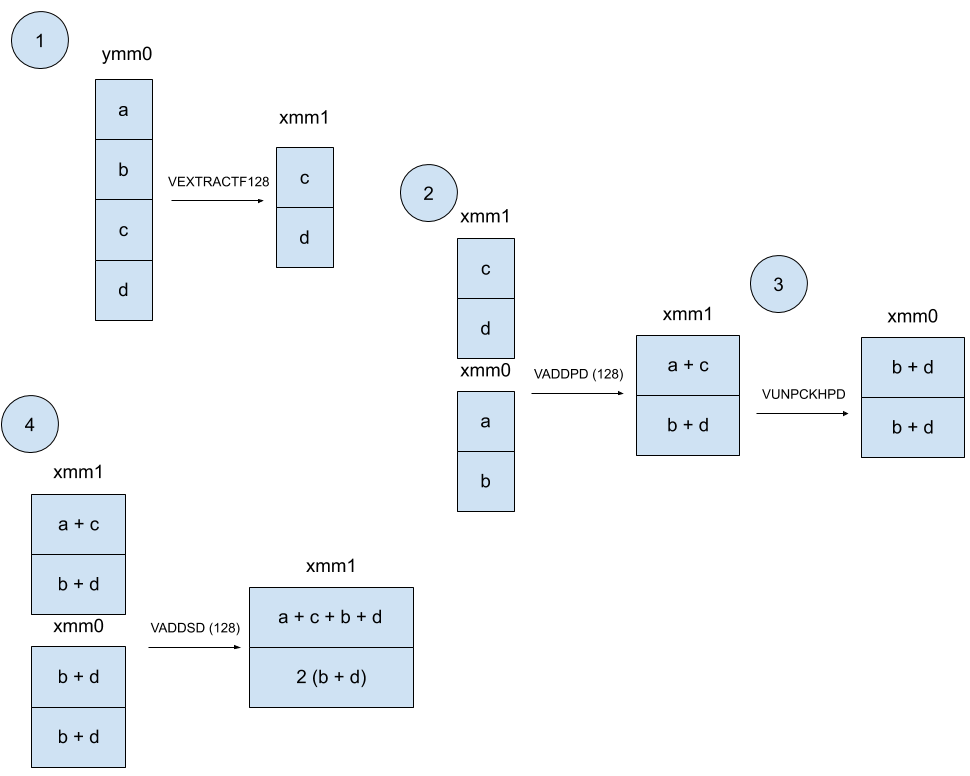
\includegraphics[width=\textwidth]{sum.png}


Since we did not want to modify the memory allocation in MLKit too much, we have made the decision to rely on the unaligned memory operations that are possible in AVX2. They might be a little slower than making sure that all accesses are properly aligned.

\subsection{Unboxing}

Since our representation of vectors is boxed, then we will have quite a large overhead doing any operations on them. Every time we want to operate on a vector we have to unbox it, do the operation and box the result. That is quite costly. In order to generate efficient machine code, we want to get rid of unnessecary boxing operations. We will do two fairly simple optimizations for now.

\paragraph{Elimination of box-unbox and unbox-box}
If we do a series of vector operations in a row, we will have box and unbox operations in between. These can be easily eliminated by considering the equivalences
\[
    \mathtt{box} (\mathtt{unbox}\ x) \equiv x
\]
and
\[
    \mathtt{unbox} (\mathtt{box}\ x) \equiv x
\]
that we assume to hold for our boxing operations. The explicit unboxing and boxing of, say, compiling $(x + y) * (a + b)$ might give us the program 
\begin{lstlisting}
box ( mul ( unbox (box (add (unbox x, unbox y)))
          , unbox (box (add (unbox a, unbox b)))
          ))
\end{lstlisting}
We can then safely rewrite this to
\begin{lstlisting}
box ( mul ( add (unbox x, unbox y)
          , add (unbox a, unbox b)
          ))
\end{lstlisting}
Eliminating 4 boxing and unboxing operations.

\paragraph{Unbox let-binding of vectors}
The explicit boxing and unboxing might leave us with a program like
\begin{lstlisting}
let
  val a = box (add (unbox x, unbox y))
  val b = box (mul (unbox x, unbox y))
in box (sub (unbox a, div (unbox b, unbox a)))
end
\end{lstlisting}
This has a lot of unnessecary boxing operations that the previous optimization did not get rid of. If we know that a boxed let-binding is always used in a unbox operation it its scope, then we can safely eliminate those operations. Then we can rewrite the previous program to
\begin{lstlisting}
let
  val a = add (unbox x, unbox y)
  val b = mul (unbox x, unbox y)
in box (sub (a, div (b, a)))
end
\end{lstlisting}
Which eliminates 5 boxing and unboxing operations and will give us fairly efficient straight-line machine code. These two optimizations are implemented in the optimizer for MLKits intermediate language.

\subsection{Signature using primops}

6. Implement the REAL4 signature using the primops.

Since our boxed representation is the same as for unboxed arrays of reals, we can use the \verb!__blockf64! primop for making vector from tuples. Similarly we can index into the vector using the \verb!__blockf64_sub_real! primop.

All the scalar operations can be implemented using the vector version combined with broadcast.
\begin{lstlisting}[frame=single]
structure M256d :> REAL4 = struct
  type m256d = string
  type simd = m256d
  type mask = m256d
  type interface = real * real * real * real

  fun mk (v: interface): m256d = prim("__blockf64", v)
  fun index (v: m256d, i: int): real = prim("__blockf64_sub_real", (v, i))
  fun read (v: m256d): interface =
    (index (v,0), index (v,1), index (v,2), index (v,3))

  fun broadcast (v: real): m256d = prim("__m256d_broadcast", v)
  fun add (a: m256d, b: m256d): m256d = prim("__m256d_plus", (a,b))
  fun adds (a: m256d, b: real): m256d = add(a, broadcast b)

  (* And so on *)
 end
\end{lstlisting}

\section{Data-parallel programming}

Using the unboxed real array from MLKit, we implement vectorized traversals.

\section{Evaluation}

\subsection{Inspecting assembly code from example programs}

We make som functions that calls the primops with the right types.
\begin{lstlisting}
type m256d = string
fun broadcast (a: real): m256d = prim("__m256d_broadcast", a)
fun add (a: m256d, b: m256d): m256d = prim("__m256d_plus", (a, b))
fun adds (a: m256d, b: real): m256d = add(a, broadcast(b))

fun mul (a: m256d, b: m256d): m256d = prim("__m256d_mul", (a, b))
fun muls (a: m256d, b: real): m256d = mul(a, broadcast(b))

fun sub (a: m256d, b: m256d): m256d = prim("__m256d_minus", (a, b))
fun subs (a: m256d, b: real): m256d = sub(a, broadcast(b))
\end{lstlisting}
A simple example program only consisting of arithmetic operations.
\begin{lstlisting}
fun g (x: m256d) = add (x, mk (0.0, 1.0, 2.0, 3.0))
fun f () =
let
  val a: m256d = mk (10.0, 20.0, 30.0, 40.0)
  val b: m256d = mul (a, a)
  val c: m256d = adds (b, 3.0)
  val d: m256d = sub (c, a)
  val e: m256d = g d
in 
  e
end
\end{lstlisting}
The core of the generated assembly code is the following
Disregarding the loading of vector literals, the resulting code is fully unboxed and just has a series of vector instructions.

For branching we want to print 1.0 if any of the elements of \verb!x! are greater than their corresponding element in \verb!y! and 0.0 otherwise.

\begin{lstlisting}
fun gt (a: simd, b: simd): mask = prim("__m256d_greater", (a,b))
fun any (a: mask): bool = prim("__m256d_any", a)
let
  val x = mk (2.0, 3.0, 4.0, 5.0)
  val y = mk (3.0, 3.0, 3.0, 3.0)
  val b = any (gt (x, y))
in 
  if b then printReal 1.0 else printReal 0.0
end
\end{lstlisting}

This generates the following code

\begin{verbatim}
  # Code to load x into ymm8 y into ymm12 above
  vcmppd $0xE,%ymm8,%ymm12,%ymm8
  vmovmskpd %ymm8,%rax
  cmpq $0x0,%rax
  movq $1,%rax
  movq $3,%r10
  cmovne %r10,%rax
  cmpq $3,%rax
  jne .LLab.newSelLab436branch.auto.mlbbranch.sml1
  movq $DLab.FloatLab32437branch.auto.mlbbranch.sml1,%rdi
  call printReal
  jmp .LLab.exitSwitchLab434branch.auto.mlbbranch.sml1
  .p2align 0x4
.LLab.newSelLab436branch.auto.mlbbranch.sml1:
  movq $DLab.FloatLab31435branch.auto.mlbbranch.sml1,%rdi
  call printReal
  .p2align 0x4
.LLab.exitSwitchLab434branch.auto.mlbbranch.sml1:
\end{verbatim}

Again fully unboxed.

\subsection{Benchmarks}

In this section we will benchmark small example programs and try to explain why they are fast, or why in some cases they are slower than expected.

\url{https://www.agner.org/optimize/blog/read.php?i=838}

Using \texttt{RealTable}\footnote{\url{https://github.com/melsman/mlkit/blob/master/basis/RealTable.sml}}

\subsubsection{Arithmetic}

For the first case we will consider modifying an array $[x_1, \ldots, x_n]$ to $[x_1(x_1 + 2), \ldots, x_n(x_n + 2)]$. The code to beat is:
\begin{lstlisting}
RealTable.modify (fun x => x * (x + 2.0)) t
\end{lstlisting}

We consider two versions. One that will make a scalar addition, which will do a broadcast with $2.0$ for each iteration:
\begin{lstlisting}
RealTable.modify_simd (fun x => mul (x, adds (x, 2.0))) t
\end{lstlisting}
The second one will store a vector $\{ 2.0, 2.0, 2.0, 2.0 \}$, and do vector addition for each iteration. This will require a memory operation instead of a broadcast.
\begin{lstlisting}
let
  val two = broadcast 2.0
in
  RealTable.modify_simd (fun x => mul (x, add (x, two))) t
end
\end{lstlisting}
The result for various array sizes are for AMD Ryzen:
\begin{center}
\begin{tabular}{ c c c c }
    Elements & Scalar (ms) & Vector 1 & Vector 2 (ms) \\
    $10^4$ & $0.015$ & $0.312$ & $0.006$ \\
    $10^5$ & $0.182$ & $2.787$ & $0.042$ \\
    $10^6$ & $1.013$ & $18.494$ & $0.489$ \\
    $10^7$ & $17.518$ & $216.674$ & $7.184$ \\
    $10^8$ & $182.967$ & $2175.133$ & $74.729$ \\
\end{tabular}
\end{center}

The result for various array sizes are for Intel i5:
\begin{center}
\begin{tabular}{ c c c c }
    Elements & Scalar (ms) & Vector 1 & Vector 2 (ms) \\
    $10^4$ & $0.121$ & $0.043$ & $0.028$ \\
    $10^5$ & $1.262$ & $0.758$ & $0.290$ \\
    $10^6$ & $6.000$ & $4.361$ & $1.027$ \\
    $10^7$ & $33.639$ & $21.238$ & $12.373$ \\
    $10^8$ & $354.351$ & $166.834$ & $119.857$ \\
\end{tabular}
\end{center}

It turns out that 

\subsubsection{Mandelbrot}

\subsubsection{Conditionals}

\begin{lstlisting}
RealTable.modify (fun x => if x > 4096.0 then x else x * x) t
\end{lstlisting}

\begin{lstlisting}
let val y = broadcast 4096.0
in RealTable.modify_simd
    (fun x => Simd4.blend (Simd4.mul (x, x), x, Simd4.gt (x, y)))
    t
\end{lstlisting}

\begin{center}
\begin{tabular}{ c c c }
    Elements & Scalar (ms) & Vector (ms) \\
    $10^4$ & $0.125$ & $0.005$ \\
    $10^5$ & $1.332$ & $0.051$ \\
    $10^6$ & $7.203$ & $0.453$ \\
    $10^7$ & $70.075$ & $7.250$
\end{tabular}
\end{center}

But this bechmark is a little misleading, since it uses a conditional move instruction instead of jumps, and therefore is highly efficient on modern hardware. The speed is of the vectorized version is comparable to the aritmetic program from before.

\section{Future work}

Aligned memory accesses

Unboxed tail recursive functions for tight loops. Take for instance a sum function

\begin{lstlisting}
foldl Simd4.add (Simd4.broadcast) arr
\end{lstlisting}

foldl will probably be tailrecursively with a vector accumulator. This is the common way to do it. The problem is that we have to box and unbox for every 4 elements. The current boxing implementation is very expensive.

Common subexpression elimination to reduce unboxing load.

Consider the function \texttt{foo}
\begin{lstlisting}
fun foo (x: m256d) =
  let
    val y = add (x, broadcast 2.0)
    val z = foo x
  in mul (z, x) end
\end{lstlisting}

\texttt{foo} will have an unbox for each occurence of \texttt{x} in arithmetic operations. It would be better to make \texttt{val x' = unbox x} available in the scope, and then replace occurences of \texttt{unbox x} with \texttt{x'} when the boxed versions are expanded. This will require a bit more complicated analysis of the program. It might be combined with common subexpression elimination.

The optimizer cannot really recognize the boxed vectors, since they just are represented using a string type. Therefore there are cases where spurious unboxes are put in the program. It is also possible to use string operations directly on a boxed vector, which is not disirable.

If the last operation is a box, then the instruction should write directly to memory instead of doing a move. Peephole optimization.

\section{Conclusion}

AMD is fucked.


\bibliographystyle{unsrt}
\bibliography{simd}

\end{document}
